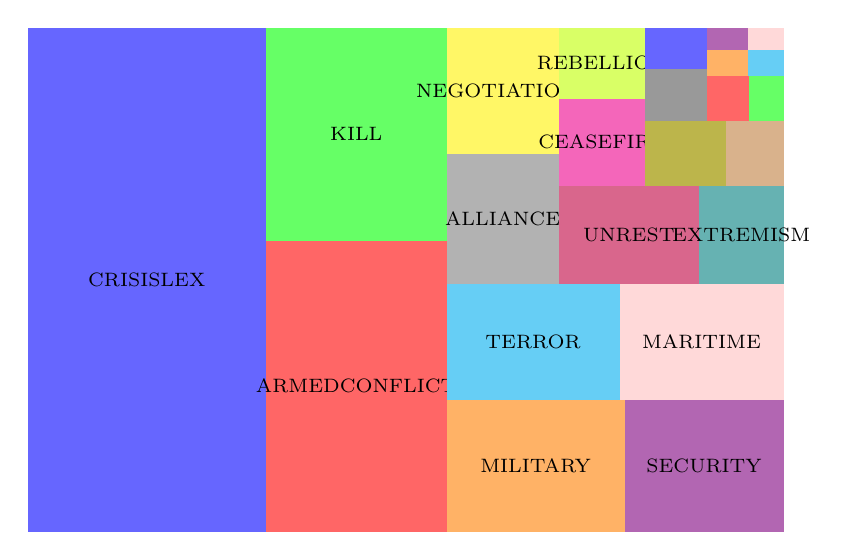
\begin{tikzpicture}[x=0.08cm,y=0.08cm]
% Auto-generated squarified treemap
% Data: 23 items, total value: 11,807,242
\fill[blue!60] (0.00,0.00) rectangle (37.82,80.00);
\node[align=center,font=\scriptsize] at (18.91,40.00) {CRISISLEX};
\fill[red!60] (37.82,0.00) rectangle (66.49,46.18);
\node[align=center,font=\scriptsize] at (52.16,23.09) {ARMEDCONFLICT};
\fill[green!60] (37.82,46.18) rectangle (66.49,80.00);
\node[align=center,font=\scriptsize] at (52.16,63.09) {KILL};
\fill[orange!60] (66.49,0.00) rectangle (94.76,20.83);
\node[align=center,font=\scriptsize] at (80.63,10.41) {MILITARY};
\fill[violet!60] (94.76,0.00) rectangle (120.00,20.83);
\node[align=center,font=\scriptsize] at (107.38,10.41) {SECURITY};
\fill[cyan!60] (66.49,20.83) rectangle (93.96,39.27);
\node[align=center,font=\scriptsize] at (80.23,30.05) {TERROR};
\fill[pink!60] (93.96,20.83) rectangle (120.00,39.27);
\node[align=center,font=\scriptsize] at (106.98,30.05) {MARITIME};
\fill[gray!60] (66.49,39.27) rectangle (84.31,59.93);
\node[align=center,font=\scriptsize] at (75.40,49.60) {ALLIANCE};
\fill[yellow!60] (66.49,59.93) rectangle (84.31,80.00);
\node[align=center,font=\scriptsize] at (75.40,69.97) {NEGOTIATIONS};
\fill[purple!60] (84.31,39.27) rectangle (106.54,54.92);
\node[align=center,font=\scriptsize] at (95.43,47.10) {UNREST};
\fill[teal!60] (106.54,39.27) rectangle (120.00,54.92);
\node[align=center,font=\scriptsize] at (113.27,47.10) {EXTREMISM};
\fill[magenta!60] (84.31,54.92) rectangle (98.01,68.74);
\node[align=center,font=\scriptsize] at (91.16,61.83) {CEASEFIRE};
\fill[lime!60] (84.31,68.74) rectangle (98.01,80.00);
\node[align=center,font=\scriptsize] at (91.16,74.37) {REBELLION};
\fill[olive!60] (98.01,54.92) rectangle (110.84,65.18);
\fill[brown!60] (110.84,54.92) rectangle (120.00,65.18);
\fill[black!40] (98.01,65.18) rectangle (107.86,73.45);
\fill[blue!60] (98.01,73.45) rectangle (107.86,80.00);
\fill[red!60] (107.86,65.18) rectangle (114.57,72.31);
\fill[green!60] (114.57,65.18) rectangle (120.00,72.31);
\fill[orange!60] (107.86,72.31) rectangle (114.42,76.38);
\fill[violet!60] (107.86,76.38) rectangle (114.42,80.00);
\fill[cyan!60] (114.42,72.31) rectangle (120.00,76.46);
\fill[pink!60] (114.42,76.46) rectangle (120.00,80.00);
\end{tikzpicture}